\documentclass[12pt]{article}

% packages

\usepackage{geometry}
\usepackage{amsmath}
\usepackage{amsfonts}
\usepackage{amsmath,amsthm,amssymb}
\usepackage{graphicx}
\usepackage{float}
\usepackage[final]{pdfpages}

% custom commands
\newcommand{\Q}[1]{\subsubsection*{Problem #1}}
\DeclareMathOperator{\epi}{epi}
\DeclareMathOperator{\dom}{dom}
\DeclareMathOperator{\diag}{diag}
\newtheorem{theorem}{Theorem}[section]
\newtheorem{lemma}[theorem]{Lemma}
% parameters
\geometry{hmargin=1cm,vmargin=1cm}
\title{ORF524 - Final Exam}
\author{Bachir EL KHADIR }

\begin{document}

\maketitle

\Q{1}
\begin{enumerate}
\item[1.] True
\item[2.] False
\item[3.] False
\item[4.] True 
\item[5.] True
\item[6.] True
\end{enumerate}

\Q{2}
\begin{enumerate}
\item[1.]
  \textbf{True}.
  
  Let's write the optimization problem in the following form:
  
  \begin{equation*}
    \begin{aligned}
      & \underset{x}{\text{min}}
      & & c^Tx \\
      & \text{subject to}
      & & Ax = b, \; x \ge 0
    \end{aligned}
  \end{equation*}
  We can assume, without loss of generality, that the problem is non-degenerate by removing some rows from $A = (A_B \; A_N)$.
  
  If a vertex $x = (x_B \; x_N)= (x_B \; 0)$ has an objective value no larger than the objective value of all its neighbours, its reduced vector cost $\bar c = c_N - c_B^TA_B^{-1}A_N$ is non negative.
  \begin{proof}    
    Let $j \in N$.  Let $d$ be a direction such that: $Ad = 0$ and $\forall i \in N \; d_i = 1_{i = j}$, eg:
    $d = (-A_B^{-1}A_j; 0, .., \underbrace{1}_j, .., 0)$.
    Then moving along the direction $\theta d, \theta \in \mathbb R^+$
    we will eventually set one coordinate in $B$ to $0$  since the feasible set is bounded, therefore reaching a neighbouring vertex.
    Let's call $\theta^*$ the maximal move in that direction($>0$ by non-degeneracy).  The change to the objective value is then  $\theta^*  \bar c_j$, which should be non-negative, and therefore $\bar c_j \ge 0$ ,and $c_N \ge c_B^TA_B^{-1}A_N$
  \end{proof}
    
  Now let $y = (y_B; \; y_N) = (A_B^{-1}(b - A_N^{-1}y_N); \; y_N)$ be a feasible point, then
  \begin{align*}
    c^T (y-x) &= c_B^T(y_B - x_B) + c_N y_N 
    \\&\ge c_B^T (A_B^{-1}(b - A_N^{-1}y_N) - A_B^{-1}b) + c_B^TA_B^{-1}A_Ny_N &\text{(since $y_N \ge 0$ and $\bar c \ge 0$)}
    \\&\ge 0
  \end{align*}
Therefore $x$ is optimal.
  
\item[2.]
  \textbf{True}.
  
  Let $\lambda \in (0, 1)$, $c_1, c_2, c, b_1, b_2, b \in \mathbb R^n$ so that $c = \lambda c_1 + (1-\lambda)c_2, b = \lambda b_1 + (1-\lambda)b_2$
  \begin{itemize}
  \item
    Convexity in $c$:
    
    \begin{lemma}
      For two sets $A, B$, if $a, b \in A, B$, then $\lambda a \le \lambda \sup A$, $a + b \le \sup A + \sup B$, so that $\sup(A + B) \le \sup A + \sup B$ and $\sup \lambda A \le \lambda \sup A$.
    \end{lemma}

    \begin{align*}
      V(b, \lambda c_1 + (1-\lambda)c_2) &= \max_{Ax \le b, x \ge 0} \lambda c_1^T x +  (1-\lambda) c_2^Tx
      \\&\le \max_{Ax \le b, x \ge 0} \lambda c_1^T x + \max_{Ax \le b, x \ge 0} (1-\lambda) c_2^Tx
      \\&\le \lambda \max_{Ax \le b, x \ge 0} c_1^T x + (1-\lambda) \max_{Ax \le b, x \ge 0} c_2^Tx
      \\&= \lambda V(b, c_1) + (1-\lambda)V(b,c_2)
    \end{align*}

  \item Concavity in $b$:
    
    Let $x_i$ be a feasible solution to $\max_{Ax_i \le b_i, x_i \ge 0} c^Tx_i$ for $i = 1, 2$.
    Then $x = \lambda x_1 + (1-\lambda)x_2$ is a feasible solution to $\max_{Ax \le b, x \ge 0} c^Tx$, and we have that $\lambda c^Tx_1 + (1-\lambda)c^Tx_2 = c^T x$
    Which means that $\max_{Ax_i \le b_i, x_i \ge 0, i = 1, 2} \lambda c^Tx_1 + (1-\lambda) c^Tx_2 \le \max_{Ax \le b, x \ge 0} c^Tx$
    Since the  $\max$ on the left invloves two independent variables, it can be distributed so that we have:
    $$\lambda V(b_1, c) + (1-\lambda) V(b_2, c) \le V(b, c)$$
    
  \end{itemize}
\item[3.]
  \textbf{False}.
  
  Take $f(x) = 1_{x > 0}$, the $\epi f = (-\infty, 0] \times [0, \infty) \cup [0, \infty) \times [1, \infty)$, which is close as the union of two closed sets, but $f$ is not continuous.
\item[4.]
  \textbf{False}.
  Take $f(x) = 1_{x > 0} \frac{1}{x} + 1_{x \le 0} \infty$

  $\epi f$ is closed but  $\dom(f) = (0, \infty)$ is not closed.

\item[5.]
  \textbf{False}.
  $f(n, -n) \rightarrow_{n \infty} 0$, but $||(n, -n)|| \rightarrow_n \infty$, so $f$ is not coercive.


\item[6.]
  
  \textbf{True}.

  Without loss of generality, by expressing the problem in an appropriate basis $(e_1, ..., e_n)$, we can assume that $Q$ is diagonal $\diag(\lambda_1, ... , \lambda_n)$ with $\lambda_1 \ge ... \ge \lambda_n \ge 0$
  
  \begin{itemize}
  \item If there exist $i$ such that $\lambda_i = 0$ and $b_i \ne 0$, then $Qe_n = 0$ and $f(\alpha e_n) = \alpha b_n \rightarrow_{\alpha \rightarrow \pm \infty} -\infty = f^*$, and the inequality is trivially verified.
    Otherwise, we can just dismiss the coordinates for which $\lambda_i = b_i = 0$ because they don't affect the objective function nor the gradient, so that we can assume $Q$ is invertible.
  \item Else, $Q$ is invertible
    $$f(x) = \frac12 (x+Q^{-1}b)'Q(x+Q^{-1}b) - \frac12 b'Q^{-1}b \ge - \frac12 b'Q^{-1}b = f(-Q^{-1}b) = f^* $$

    We have that:
    $$x_{k+1} = x_k - \alpha \nabla f(x_k)
    = x_k - \alpha Q(x_k+bQ^{-1})$$

    Adding $bQ^{-1}$ to both sides:
    $$x_{k+1}+Q^{-1}b = (I - \alpha Q) (x_k +Q^{-1}b)$$
    So:
    $$||x_{k+1}+Q^{-1}b||^2 \le ||I-\alpha Q||^2 ||x_k + Q^{-1}b||^2$$
    Therefore
    $$f(x_{k+1}) - f^* \le \rho (f(x_k) - f^*)$$

    By immediate induction, $f(x_k) - f^* \le \rho^k (f(x_0) - f^*)$ with $\rho := ||I-\alpha Q||^2$.
    
    For $\alpha$ small enough, the eigen values of $(I - \alpha Q)$ are all smaller than $1$, and $\rho < 1$
  \end{itemize}
  
\end{enumerate}

\Q{3}
\begin{enumerate}
\item The dual problem:

  \begin{equation*}
    \begin{aligned}
      & \underset{y}{\text{maximize}}
      & & (1+\lambda)y_1 + (-2+\lambda)y_2 + (2 + \lambda)y_3 + (5+\lambda)y_4 \\
      & \text{subject to}
      & & y_1 + y_2 \le -4 -\lambda \\
      & & & -y_1 + 2y_2  - y_3 \le 3 - 2\lambda \\
      & & & -y_1 + y_2  - y_4 \le 1 - \lambda \\
    \end{aligned}
  \end{equation*}

  Complementary conditions:
  \begin{align*}
    (1 + \lambda + x_1 - x_2 - x_3)y_1 &= 0 \\
    (-2 + \lambda + x_1 + 2x_2 + x_3)y_2 &= 0 \\
    (2 + \lambda - x_2)y_3 &= 0 \\
    (5 + \lambda - x_3)y_4 &= 0 \\
  \end{align*}

\item
  $$\lambda \ge 2$$
  \[
    \begin{array}{c|c|c|c|c}
      V(\lambda) = 0 & (-4-\lambda) x_1 &+ (3-2\lambda)x_2 &+ (1-\lambda)x_3\\
      \hline
      w_1 = 1+\lambda      & 1          & -1         &-1        \\
      w_2 =-2+\lambda      & 1          &  2         & 1        \\
      w_3 = 2+\lambda      & 0          &  -1        & 0        \\
      w_4 = 5+\lambda      & 0          &  0         & -1       \\
    \end{array}
  \]
  
  $$\frac{3}{2} \le\lambda \le 2$$
  \[
    \begin{array}{c|c|c|c|c}
      V(\lambda) = -\frac12 (-2+\lambda)(3-2\lambda) &  x_1 &+ w_2 &+ x_3\\
      \hline
    \end{array}
  \]

  $$ \frac32 \ge \lambda \ge 0$$
  \[
    \begin{array}{l|c|c|c|c}
      V(\lambda) = (3-2\lambda)(1+\lambda) & (-1-3\lambda) x_1 &- (3-2\lambda)z_1 &+ (3\lambda-2)x_3\\
      \hline
      x_2 = 1+\lambda         & 1          &  -1        &-1        \\
      w_2 = 3\lambda          & 3          &  2         & -1        \\
      w_3 = 1           & -1          & 1         & 1        \\
      w_4 = 5+\lambda         & 0          &  0         & -1       \\
    \end{array}
  \]

\item  

  \[
    V(\lambda) =
    \left\{
      \begin{array}{cl}
        0           & \text{if $2 \le \lambda$}\\
        -\frac12 (-2+\lambda)(3-2\lambda)& \text{if $\frac{3}{2} \le \lambda\le 2$}\\
        (3-2\lambda)(1+\lambda) & \text{if $0 \le \lambda \le \frac 32$}\\
      \end{array}
    \right.
  \]

  \begin{figure}[H]
    \centering
    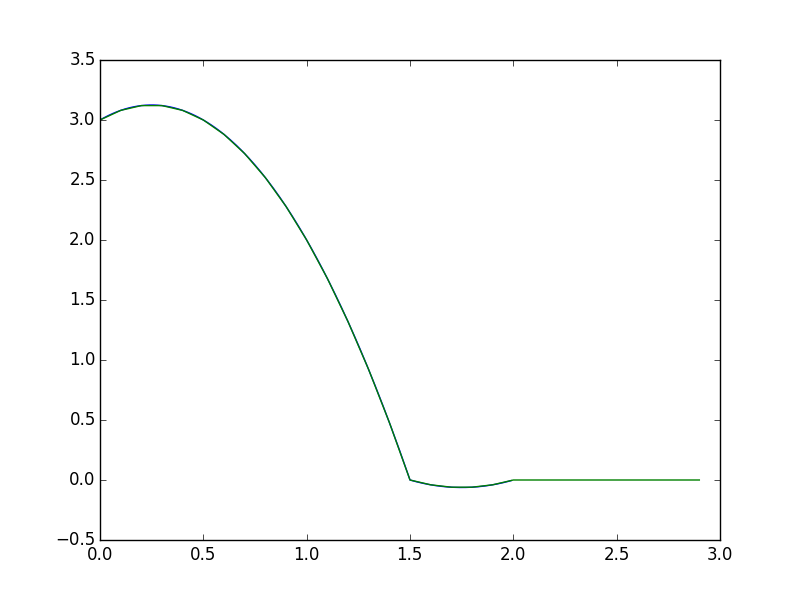
\includegraphics[width=0.5\textwidth]{q3.png}
  \caption{$V(\lambda)$}
  \end{figure}

\item
  \[
    V'(\lambda) =
    \left\{
      \begin{array}{cl}
        0           & \text{if $\frac 2 < \lambda$}\\
        2\lambda - \frac72           & \text{if $\frac 32 < \lambda < 2$}\\
        -2\lambda+1 & \text{if $0 \le \lambda < \frac 32$}\\
      \end{array}
    \right.
  \]
  In $2$ and $\frac{3}{2}$, $V$ has only right and left derivative.
  $V'(2+) = 0, V'(2-) = \frac12, V'(\frac32+) = -\frac12, V'(\frac32-) = -2$
\end{enumerate}

\Q{4}

\begin{enumerate}
\item
  
  
  If $x, y \in \{0, 1\}$, then $x^2 + y^2 = x+y \in \{0, 1, 2\}$.
  Let $v := x + y$, then :
  \[
    p(u) = \min_{a-u \le v, \; v\in\{0, 1, 2\}} v =\left\{
      \begin{array}{ll}
        0 & \text{if $a \le u$}\\
        1 & \text{if $a - 1 \le u < a$}\\
        2 & \text{if $a - 2 \le u < a-1$}\\
        \infty & \text{if $u < a - 2$}\\
      \end{array}
    \right.
  \]
  The problem is not convexe because the feasible set is discrete and not reduced to a singleton.
  $p$ is non-increasing, so it has a right limit everywhere, furthermore it is right-continuous, so: $\lim \inf_{x \rightarrow x_0} f(x) = \lim_{x \ge x_0}f(x) = f(x_0)$, so it is lower semi-continuous.


    \begin{figure}[H]
    \centering
    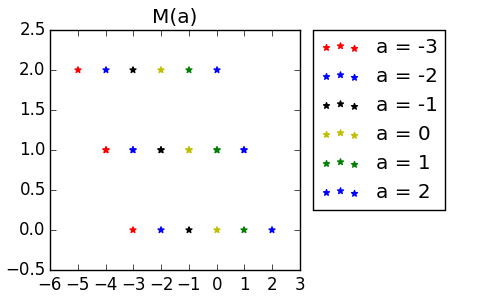
\includegraphics[width=0.5\textwidth]{sketch.png}
    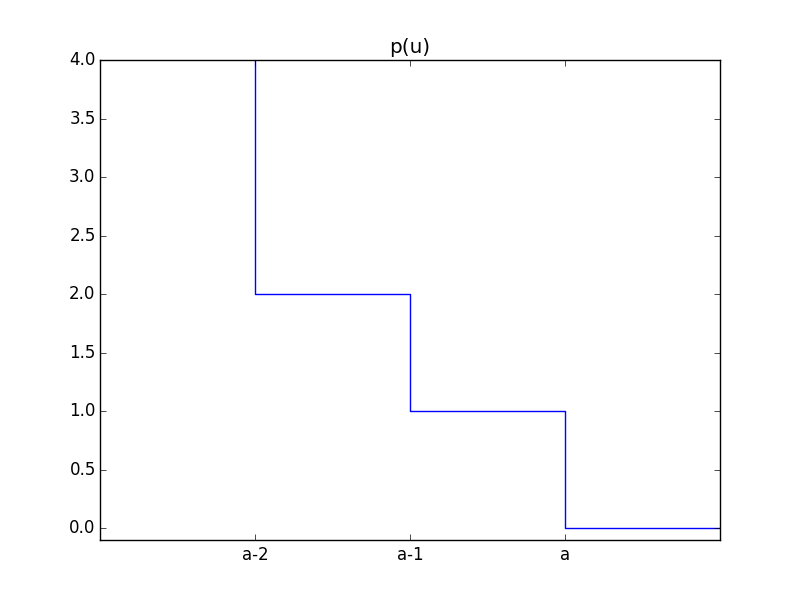
\includegraphics[width=0.5\textwidth]{pu.png}
    \caption{Sketch of $\bar M(a)$ and $p(u)$}
  \end{figure}

  
\item
  The problem is feasible iff $a \le 2$

  In the following graph I have drawn the supporting (and non parallel to the $y$ axis) hyperplanes of $\epi p$.

    \begin{figure}[H]
    \centering
    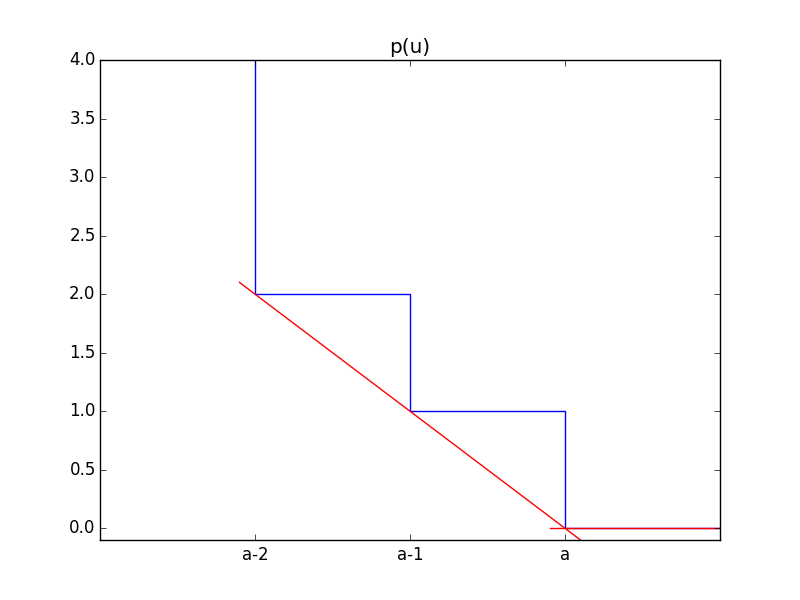
\includegraphics[width=0.5\textwidth]{support.png}
    \caption{Supports of $\epi(p)$}
  \end{figure}

  
  \begin{itemize}
  \item The primal equals to the dual when the min common
    point of the $y-axis$ equals the max crossing support, ie when
    $a \le 0$ or $a \in \{1, 2\}$.

  \item There is a duality gap otherwise, ie when
    $a \in (0, 2) \setminus \{1\}$
  
  \item There is uniqueness of the dual solution only if there is a unique supporting plane crossing the $y-$axis at a maximal point. It is the case whenever $a \ne 0, a \le 2$.
  \end{itemize}
\item Take $a = -1$.
  Let $X = \{0,1\}$
  The primal: $$\max_{x+y \ge -1, x, y \in X} x^2 + y^2$$, the optimal value is $0$, and the optimal solution is $(0, 0)$
  
  The dual:
  \begin{align*}
    \min_{\lambda \le 0}  \max_{x, y \in X} -\lambda (1+x+y) + x^2 + y^2
    &= \min_{\lambda \le 0} 2\left(\max_x x^2 - \lambda x\right) - \lambda\ &\text{(By symmetry)}
    \\&= \min_{\lambda \le 0} - \lambda + 2\max_{x \in \{0, 1\}} x (1-\lambda)  &(x^2 = x)
    \\&= \min_{\lambda \le 0} - \lambda + 0 &(1-\lambda > 0)
    \\&= 0 &\text{(When $\lambda = 0$)}
  \end{align*}

\end{enumerate}


\Q{5}
\begin{itemize}
\item 
  \begin{itemize}
  \item States: $(i, j)$ meaning we have to do the multiplication of the matrices $M_i...M_j$, and $C(i, j)$ is the optimal cost to doing this multiplication
  \item Action: Put the parentheses at position $k \in \{i, ..., j-1\}$: $M_i...M_j = (M_i... M_k)(M_{k+1}...M_j)$
  \item Cost: The cost to doing the multiplication $(M_i... M_k)(M_{k+1}...M_j)$, is $r_ic_kc_j + C(i, k) + C(k+1, j)$
  \end{itemize}
  $$C(i, i) = 0$$
  $$C(i, j) = \min_{k = i,..,j-1} r_ic_kc_j + C(i, k) + C(k+1, j)$$
\item

  Shortest path formulation:

  \begin{itemize}
  \item Node space:  $\{ (k_{i_1}, ..., k_{i_r}) | k_{i_j} \text{ all different },r \in \{1, ..., n-1\} \}$, $(k_{i_1}, ..., k_{i_r})$ denotes the order in which we put the parentheses:
    \begin{enumerate}
    \item $(M_1 ... M_{k_{i_1}})( M_{k_{i_1+1}} ... M_n)$
    \item $( (M_1 .. M_{k_{i_2}})(M_{k_{i_2}+1} .. M_{k_{i_1}}))( M_{k_{i_1+1}} ... M_n)$ if $k_{i_2} < k_{i_1}$,
      $(M_1 ..  .. M_{k_{i_1}})( (M_{k_{i_1+1}} ... M_{k_{i_2}})(M_{k_{i_2}+1} ... M_n))$ otherwise.
    \item etc...
    \end{enumerate}
  \item Starting node: $()$ the empty tuple.
  \item Final nodes: $(k_{i_1}, ..., k_{i_{n-1}})$ tuples with $n-1$ elements.
  \item Transitions: $(k_{i_1}, ..., k_{i_r}) \rightarrow (k_{i_1}, ..., k_{i_r}, k_{i_{r+1}})$ where $k_{i_{r+1}} \not \in \{k_{i_1}, ..., k_{i_r}\}$
  \item Cost: Let $a = \max\{ k_{i_j}| k_{i_j} < k_{i_{r+1}}\}$, $b = \min\{ k_i | k_{i_j} > k_{i_{r+1}}\}$.
    The cost is then $r_ac_{k_{i_{r+1}}}r_b$
  \end{itemize}
  The problem with this formulation is that it takes an exponential number of nodes ($O(n^n)$)
  
\item Linear programming formulation:
    \begin{equation*}
    \begin{aligned}
      & \underset{D}{\text{maximize}}
      & & \sum_{i < j} D(i,j)
      & \text{subject to}
      & & D(i,j) \le r_i c_k c_j +  D(i,k) + D(k+1, j) \forall k \in \{i, ..., j-1\}
    \end{aligned}
  \end{equation*}
It is clear that $C$ is a solution to this linear problem.(see lecture 22)
\end{itemize}

\Q{6}
\begin{enumerate}
\item Look at the code.

\item
  Let $\mathcal C$ be the set of the sort trajectories, and $p = \frac1{ |\mathcal C|}$
  \begin{itemize}
  \item States: $(t, S)$
  \item Randomness: $(t, S) \rightarrow (t+1, S+s)$, $s \sim \mathcal U(\mathcal C)$.
  \item Actions: Hold / Exec
  \item Transitional cost: $0$ if we hold, $S - K$ if we exercise.
  \end{itemize}
\item Bellman equation:
  $$V_k(S) = \max\{S - K, p \sum_{s \in C} V_{k+1}(S + s) \}$$
  $$V_T(S) = (S-K)^+$$
\item
  \textbf{Value iteration:} Look at the code.
  
  \textbf{LP formualation:}
  Let $J(t, S)$ be the price of the option at time $t$ is $S_t = S$,
  and we decide to adopt the strategy 

  $J$ verifies: $J(t, S) = \max \{ E[J(t+1, S_{t+1}) | S_t = S], S - K \} = [\max_{\mu} (P_{\mu}J + g_\mu) ](t,S) $
  where:
  $$\mu(t, S) \in \{ \text{HOLD}, \text{EXEC} \}$$
  \[ (P_\mu J)(t, S) = \left\{
      \begin{array}{cc}
        p \sum_{s \in \mathcal C} J(t+1, S+s) & \text{ if $\mu(t, S) = $ HOLD } \\
        0 & \text{otherwise}
      \end{array}
    \right.
  \]
  \[
    g_\mu(t, S) = \left\{
      \begin{array}{cc}
        0 & \text{ if $\mu(t, S) = $ HOLD } \\
        S - K & \text{otherwise}
      \end{array}
    \right.
  \]

  The LP problem is:
  $$\min e^T J \text{ s.t } \forall \mu \, J \ge P_\mu J + g_\mu$$
  At time $t$, $S$ can take the following values $\{ S_{t-1} + s,\, s \in \mathcal C\} = \{ S_t^k, k \le N_t \}$ where $(S_t^k)$ is an increasing sequence. Let's denote by $\tilde J(t, k) := J(t, S_t^k)$ when $k \le N_t$ and $L$ otherewise where $L >> S_0$ is a very big constant.
  The problem can be written as:
  \begin{align*}
    \min &\sum_{t, k} \tilde J(t, k) \\
         &\text{ s.t } \forall t, k \in \{1...T-1\}\\
         & \tilde J(t, k) \ge p \sum_{j \le |\mathcal C|} \tilde J(t+1, k+j)  \\
         & \tilde J(t, k) \ge S_t^k - K\\
         & \tilde J(T, k) = S_T^k - K \\
         & \tilde J(t, k) = L \text{ when } k > N_t\\
  \end{align*}

  Let $x_{t*T + k} = \tilde J(t, k)$, and define $A \in \mathcal M_{T^2, T^2}$,
  $B \in \mathcal M_{\frac{T(T-1)}{2}, T^2}$ $U \in \mathbb R^{T^2}$ such that:

  \[
    A := 
    \begin{array}{r@{}}
      \text{T(T-1)}~\left\{\begin{array}{@{}c@{}}\null\\\null\\\null\end{array}\right.\\
      \text{T}~\left\{\begin{array}{@{}c@{}}\null\\\null\end{array}\right.\\
    \end{array}
  \left [
    \begin{array}{ccccc}
      0               & p                     & ...  & p     & \cdots \\
      \vdots          &                       & \ddots & \ddots& \cdots \\
      0               &                       & \cdots & p     & p  \\
      0               & 0                     & 0      & 0     & 0      \\
                      & \cdots                & \cdots &       & 
    \end{array}
  \right ]
\]


  \[
    B := 
    \begin{array}{r@{}}
      \text{T-1}~\left\{\begin{array}{@{}c@{}}\null\\\null\\\null\end{array}\right.\\
      T-N_1~\left\{\begin{array}{@{}c@{}}\null\\\null\\\null\\\null\end{array}\right.\\
      \text{\vdots}~\left\{\begin{array}{@{}c@{}}\null\end{array}\right.\\
     T - N_{T-1}~\left\{\begin{array}{@{}c@{}}\null\end{array}\right.\\
    \end{array}
  \left [
    \begin{array}{cccc|ccccc|c|ccc}
      0 & 1      &        &\cdots &&& &&& &&& \\
        &        & \ddots &       &&& &&& &&& \\
        &        &        & 1     &&& &&& &&& \\
      \hline
        &        &        &       & 0 & 0 & 1 & \cdots &   &&&&\\
        &        &        &       &   &   &   & \ddots &   &&&& \\
        &        &        &       &   &   &   &        & 1 &&&&\\
      \hline
        &        &        &       &   &   &   &        & & \ddots \\
      \hline
        &        &        &       &   &   &   &        & &        & 0 & \cdots & 1 \\
    \end{array}
  \right ]
\]
 $U \in R^{T^2}$ such that : $U_{tT + k} := S_t^k - K$

 The LP problem is equivalent to:
 \begin{align*}
    \min & e^T x \\
         &\text{ s.t } \\
         & x \ge Ax \\
         & x \ge U\\
         & Bx = L 1_{\frac{T(T-1)}2}
  \end{align*}



\end{enumerate}

\newpage
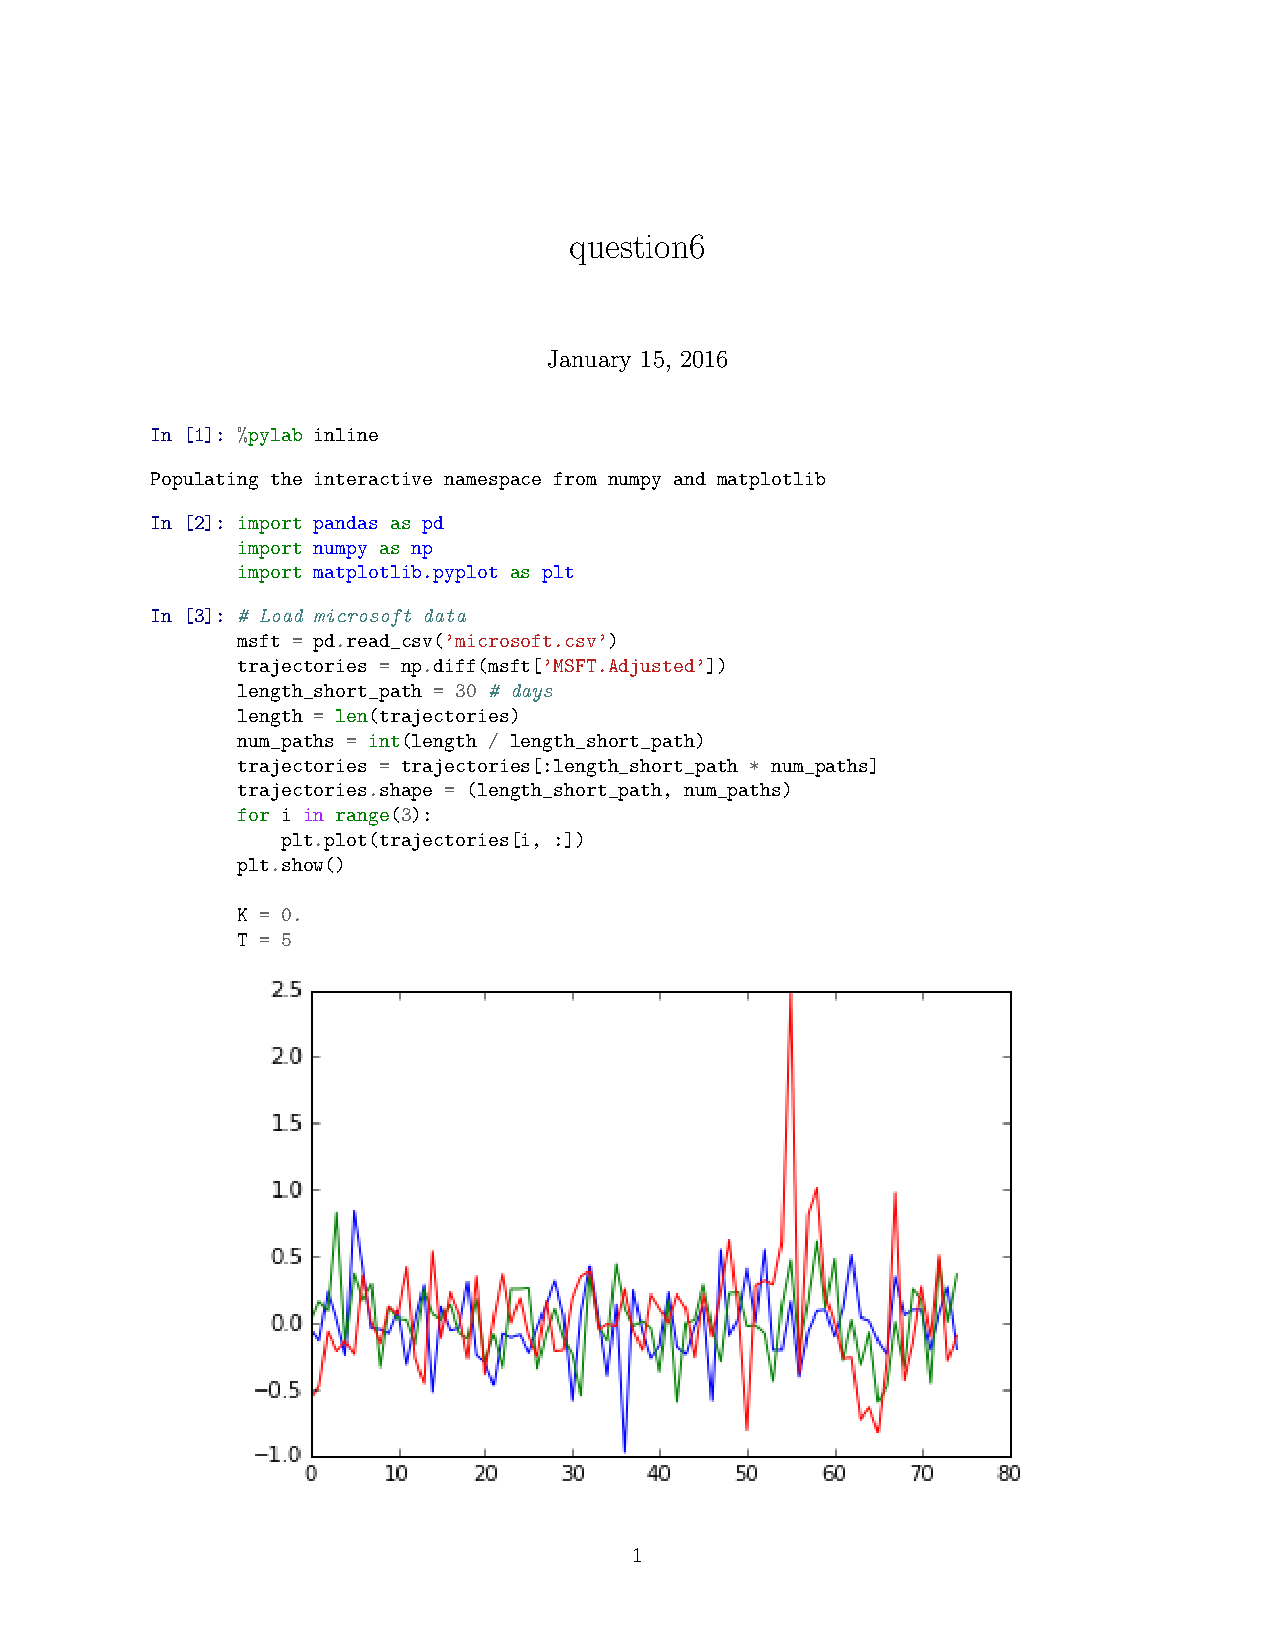
\includepdf[pages=-]{question6.pdf}


\end{document}

%%% Local Variables:
%%% mode: latex
%%% TeX-master: t
%%% End:



























